% !TeX root = ../main.tex

\chapter{绪论}

\section{研究背景和意义}

随着全球科技竞争的加剧,信息技术自主可控已成为国家战略的重要组成部分。龙芯作为国产处理器的代表,其生态系统的完善和应用推广对打破国外技术垄断、实现核心技术自主化具有重要意义。
然而,目前龙芯平台主要集中于桌面和服务器领域,在移动设备领域的应用仍处于空白或起步阶段。因此,基于龙芯平台开发移动设备相关技术,不仅是对国产处理器生态的扩展,
更是对国家信息技术自主化战略的重要支持。

而相应的,Android 系统作为全球最广泛使用的移动操作系统之一,其意义和重要性不言而喻。
根据 statcounter 的数据,2023 年11月至2024年11月全球智能手机市场中,Android 系统的市场份额均超过 70\%\cite{MobileMarket}。
这意味着大量的用户依赖于 Android 平台进行日常操作和娱乐。
\begin{figure}[h]
    \centering
    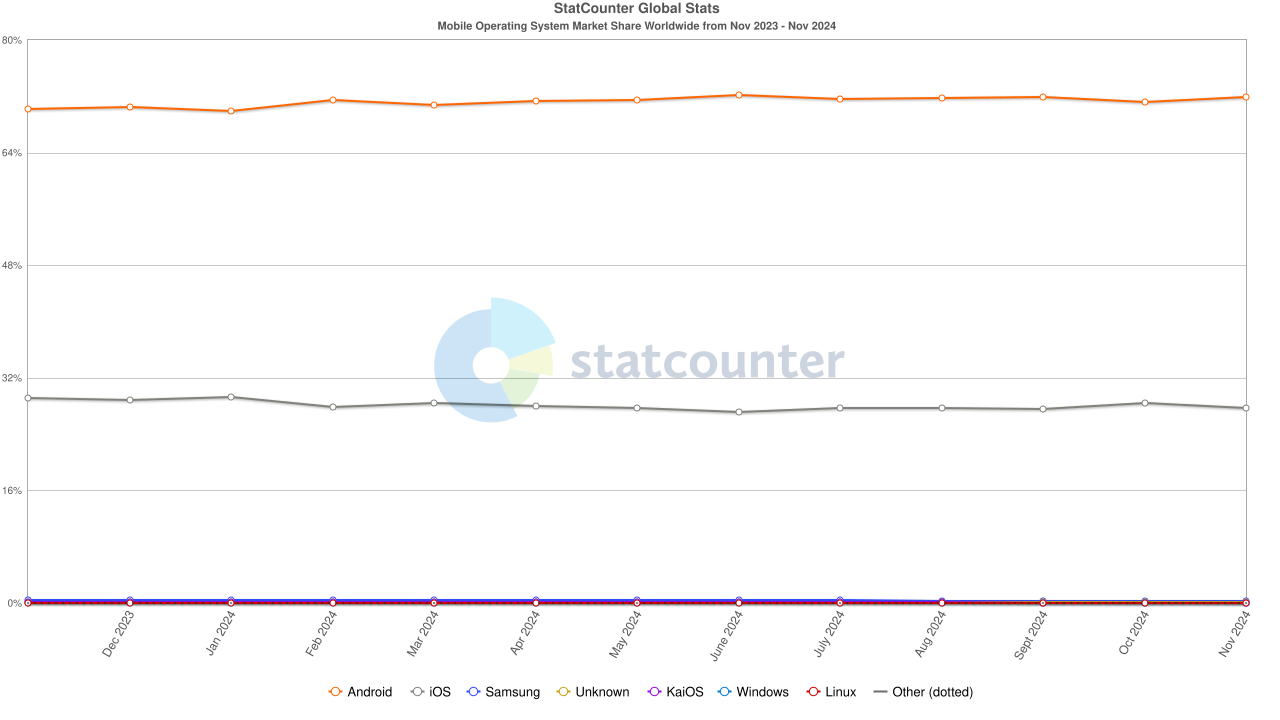
\includegraphics[width=0.8\textwidth]{2024全球智能手机市场占有率统计.png}
    \caption{2024全球智能手机操作系统市场占有率统计}\cite{MobileMarket}
  \end{figure}
Android作为Google公司开发的开源操作系统,其在国内市场也有广泛的应用领域,滋养了移动端设备的蓬勃发展。但是中美科技战的背景下,
高端移动设备的芯片进口受到限制,产业发展受制于人。龙芯作为国产自主芯片的领头羊,于2021年推出了自主指令集Loongson Architecture(LoongArch)\cite{Loongarch},
涵盖基础架构、虚拟化、向量指令等多个部分。由于龙芯目前多专注于桌面、服务器以及嵌入式领域,新型的LoongArch架构也尚未支持主流的安卓或鸿蒙等开源操作系统,
因此亟待移动端基础软件的支持以及软件生态的建设。将安卓移植到龙芯指令集上不仅有利于丰富完善龙芯的软件生态,而且会为后续的移动端国产化替代提供一个探索性的方案,
是非常有意义的。

Android 的图形系统作为Android系统最基础最重要的模块之一,图形系统的正确运行与否直接导致zygote(所有Android应用进程的起点)进行能否顺利创建。
而同时,Android图形系统又是一个极为复杂的系统,其复杂性体现在其多层架构中,包括应用层、框架层、硬件抽象层(HAL)及底层驱动。
这种多层结构使得开发者能够灵活地利用不同的图形 API,在设计上具有高度的灵活性和可扩展性,但却极大的增加了安卓框架本身的复杂性,使得在实际应用中仍面临诸多挑战。
例如,不同设备的硬件差异使得图形性能的优化变得复杂。这使得开发者需要针对不同设备进行优化,以确保应用在各种硬件上的流畅运行。
此外,Android 的多任务处理机制可能导致图形渲染时的资源竞争,进而影响应用的响应速度和帧率。这一问题在资源密集型应用中尤为明显,如大型游戏或复杂的图形应用。
研究表明,游戏应用中的帧率波动会直接影响用户的留存率,帧率是影响用户满意度的关键因素\cite{2006The}。

通过对图形系统的研究和优化,可以提高应用程序的图形渲染效率,加快界面的响应速度,降低卡顿现象的发生频率。此外
一个稳定的图形栈可以减少应用程序崩溃和系统崩溃的可能性,提高系统的稳定性和可靠性,保障
用户数据的安全性;优化应用程序的图形渲染流程,提高应用程序的性能表现,减少资源占用,降
低功耗消耗,从而提升开发效率和节约开发成本。因此,对 Android 图形栈的研究具有重要的理论和实际意义。

本课题旨在探索利用基于龙芯平台,实现一个使用龙芯国产CPU和GPU的安卓图形系统设计方案,解决龙芯安卓图形系统中极为重要的一系列基础依赖库或软件等问题,
为后续的一系列基于安卓系统的开发打下基础,推动安卓项目的顺利进行。

\section{国内外研究现状}
\subsection{移动端显卡驱动现状}
移动设备显卡驱动用于处理智能手机、平板电脑和其他移动设备的图形渲染任务。与桌面显卡驱动相比,它们在功耗和散热方面的优化尤为重要,
以确保设备的电池寿命和用户体验。移动显卡驱动的主要功能有实现低功耗优化,动态调整 GPU 的频率和电压,以节约电池电量;
图形加速,支持高效的 2D/3D 渲染,以提高用户界面和应用程序的图形性能;视频解码和编码,为高清视频和流媒体播放提供硬件加速支持;
以及高效的图形API支持,移动驱动通常支持 OpenGL ES 和 Vulkan,以实现高效的图形渲染。常见的移动设备的显卡驱动有ARM Mali驱动,
Qualcomm Adreno 驱动,Imagination PowerVR 驱动,苹果 A 系列和 M 系列芯片。

1.ARM Mali驱动\cite{ARM}:ARM Mali驱动是为ARM Mali GPU设计的一套图形处理单元驱动程序,它支持OpenGL ES、Vulkan、OpenCL等图形和计算接口,
用于嵌入式设备和移动设备的图形处理。Mali GPU广泛应用于智能手机、平板电脑、智能电视和其他嵌入式系统。已有多个GPU系列产品的配套驱动,如
Utgard、Midgard、Bifrost、Valhall等,同时有开源和闭源的驱动实现,开源实现由Panfrost、Lima等社区开发,
而闭源实现则是由ARM 官方提供的 Mali GPU 驱动。

2.Qualcomm Adreno\cite{qualcomm} 驱动:Qualcomm Adreno 是高通公司为其 Snapdragon 系列芯片设计的 GPU(图形处理单元),
广泛应用于智能手机、平板电脑和其他嵌入式设备。Adreno 驱动程序为这些设备提供图形渲染和计算能力,
支持现代图形 API(如 OpenGL ES、Vulkan 和 OpenCL),用于运行复杂的图形和计算任务。
如同Mali驱动一样,Adreno也有开源和闭源的实现。freedreno 是 Linux 社区开发的开源 Adreno 驱动,支持 OpenGL ES 和 Vulkan。
闭源实现是由Qualcomm 提供,通常嵌入到 Android 中,提供完整的 GPU 功能支持和性能优化。

3.Imagination PowerVR \cite{imaginationtech}驱动:应用于Imagination Technologies 的 PowerVR 系列 GPU,用以支持高效图形和计算解决方案以及
延迟渲染架构(Deferred Rendering Architecture),并且提供提供高效的渲染性能和低功耗的特性。该驱动被用于许多移动设备,
如部分 iPhone 和其他手机品牌。通常是闭源的,优化只针对特定硬件。

4.苹果 A 系列和 M 系列芯片\cite{apple}:适用于苹果自研的苹果的 A 系列和 M 系列芯片,A 系列主要用于 iPhone 和 iPad,
M 系列则主要用于 Mac 和 iPad,二者都基于 ARM 架构设计。该驱动程序针对苹果的硬件进行深度优化,
以提供高性能、低功耗的图形处理能力。


% 关键技术:Tiling 渲染:移动 GPU 驱动经常使用 tile-based 渲染架构来减少带宽需求和功耗。
% 异步计算:驱动程序支持异步任务,以提高图形渲染和计算任务的并行处理能力。
% 热管理:驱动程序会监控设备温度,并动态调整性能以防止过热。

% 图形模拟器?
% x11
% mesa
% gpu模拟器:gpgpu sim
% 命令队列 commandqueue

\subsection{图形系统架构优化}
由于安卓图形栈的性能与用户体验高相关,Google 本身也在对图形栈做一些优化。这一部分的优化主要是由Google公司完成。
Android 4.1之后,Google 对 Android Display 系统进行了重构,实现了黄油工程(Project Butter),在系统受到
VSync pulse 后,马上开始下一帧的渲染,称为 drawing with VSync,让 CPU/GPU 有完整的时间来处
理数据,减少了卡顿(jank),具体实现上引入了 Choreographer\cite{google2012dev}。在 Android 7.0 版本之后,首次
引入 Vulkan API,实现了低开销和高性能的特点,并且允许多线程同时提交工作到 GPU。相比较
OpenGL ES,Vulkan 在性能提升、帧率提升、cpu 使用率等方面均有较大提升。在Android 9.0 版本中,引入了
minigbm,旨在为 Android 提供更灵活的缓冲区管理,并用一种标准化的方式来管理和分配图形缓冲区,与 
Direct Rendering Manager(DRM)紧密结合,使得在 Linux 设备上进行图形输出和显示变得更加高效,满足了
嵌入式设备对性能和资源管理的严格要求。

\subsection{与非ARM架构的兼容}
由于安卓图形系统较为重要,因此有部分开源项目以及学者提供了一些方案,以期同时兼顾兼容性和高效性。以下是一些方案的介绍。
张超等\cite{张超2012Android}实现了SurfaceFlinger在桌面Linux的X Window环境下运行。其主要方法是通过替换gralloc硬件模块使用Linux上的窗口引擎,
也就是使用软件渲染的方式将SurfaceFlinger合成的图像写入共享内存,
 再由一个桌面图形程序输出画面. 该方法的不足是使用软件渲染而没有调用GPU实现硬件加速, 造成占用大量CPU时间, 并且画面输出过程需要不断调用IPC,
 在处理3D图形时只有个位数的帧数, 性能较为低下。

\begin{figure}[h]
  \centering
  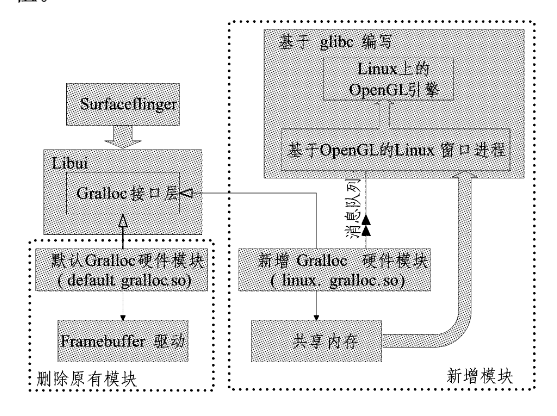
\includegraphics[width=0.8\textwidth]{Android图形系统向桌面Linux的移植.png}
  \caption{Android图形系统向桌面Linux的移植}\cite{张超2012Android}
\end{figure}

Android X86\cite{AndroidX86}项目在X86架构的PC上运行Android系统,该项目使用Mesa\cite{mesa3d}的OpenGL ES实现,并基于DRM\cite{DRM}和GEM\cite{GEM}实现了gralloc.drm模块,
成功运行了可在X86架构下运行硬件加速的SurfaceFLinger。在此基础上,江帆等\cite{XTYY201710015}提出了一种可以在X Window系统下运行Android SurfaceFlinger的方案,
具体是使用Mesa作为OpenGL ES实现并使Mesa EGL兼容Android的本地窗口,实现了能够GPU硬件加速的图形合成过程,另外使用DRI2拓展避免了图像缓存由独显到系统内存的拷贝过程。

\begin{figure}[H]
  \centering
  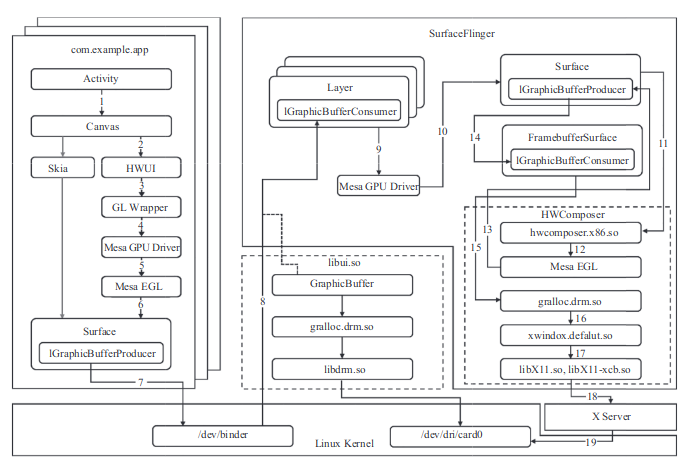
\includegraphics[width=0.8\textwidth]{SurfaceFlinger移植X环境架构.png}
  \caption{SurfaceFlinger移植X环境架构}\cite{XTYY201710015}
\end{figure}

李\cite{1016779798.nh}设计了一种新的图形系统框架,其参考了安卓图形系统的设计思想,采用分层的架构实现,包括系统平台层、系统运 行库层、应用程序框架层和应用程序层,
系统运 行库层采用 Linux 系统提供的底层库以及一些优秀的开源库,包括字体矢量、XML (Extensible Markup Language)文档解析、数据压缩解压缩、二维向量图形处理等;
应用程序框架层和应用程序层采用与安卓图形系统基本一致的资源解析、界面绘制及图 像显示流程,并且在系统运行库层和应用程序框架层进行了一定的改造优化。
\begin{figure}[H]
  \centering
  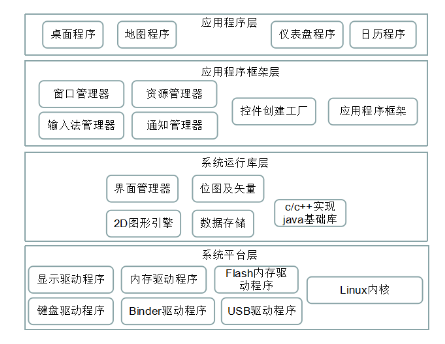
\includegraphics[width=0.6\textwidth]{cnd系统架构.png}
  \caption{cnd系统架构}\cite{1016779798.nh}
\end{figure}

高\cite{高胜寒2019基于国产}基于国产图形处理器设计了一套图形硬件抽象层。该方案对下可兼容国产化GPU硬件,对上可兼容图形API,且可支持多个操作系统。
\begin{figure}[H]
  \centering
  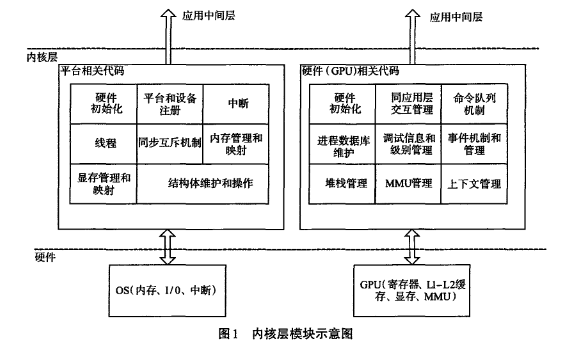
\includegraphics[width=0.6\textwidth]{高胜寒2019基于国产.png}
  \caption{高:内核层模块示意图}\cite{高胜寒2019基于国产}
\end{figure}

\section{本文主要工作}

本课题以在LoongArch架构上构建可运行的Android运行环境,并打通图形系统相关依赖,从而实现安卓上层应用可以调用运行龙芯LG110显卡的目的。
在对Android系统结构、源码以及图像系统进行分析的基础上,移植并实现了一套可以在龙芯3A5000和7A2000桥片(包含LG110显卡)上运行的安卓图形系统运行环境。
主要包括以下内容:
\begin{itemize}
  \item 学习分析Android系统的结构和图形系统的运行机制,为后续添加龙芯硬件支持打下基础
  \item 移植安卓的Native程序在LoongArch上运行环境的构建,使Android的Native程序可以在LoongArch上运行
  \item 完成基于LoongArch的安卓5.10内核和安卓12镜像的构建,包括根据目标硬件平台做了一些兼容性补丁,以支持16k page\_size等特性
  \item 完成了LG110显卡的内核驱动的多版本构建的实现,完成LG110用户态显卡驱动Mesa的移植。
  \item 重构封装龙芯安卓系统的LG110显卡的硬件抽象层,包括gralloc以及HWC等关键依赖库的移植,并打通显示通路。
\end{itemize}
%MARK:创新点依旧有待商榷。
本文的预期目标是能够在安卓平台下正确调用LG110显卡,并运行Android Native程序,在3A5000硬件平台下运行启动安卓系统并进入开机动画,并成功通过相关
程序的测试和验证。

\section{本文的组织架构}
本文第一章是绪论部分,介绍研究背景和意义,国内外研究现状,并对全文的组织结构进行阐述。

第二章围绕课题介绍了安卓图形显示的原理和相关技术,包括安卓图形系统个部分组件,如何构建安卓系统以及内核的支持等。以及龙芯
平台提供的底层支持如GPU以及固件等。

第三章着重分析安卓图形系统的整体结构,以及分析如何在龙芯平台上运行安卓图形,包括分析渲染和加载龙芯驱动的关键流程,所需的各个组件支持,以及为了适应
龙芯硬件平台所必须做的一些调整。

第四章是性能分析和优化,暂定。。。

第五章是对整个图形系统包括龙芯专有驱动在内的实现进行评估和测试,包括测试环境,功能测试,性能测试等。

第六章对论文的工作内容作了总结,分析了所构建系统的优势与不足,并对课题的未来研究方向做出了一些展望和建议。

